% setup
\documentclass[11pt]{article}
\usepackage{mathptmx} % Use Times New Roman font
\usepackage[a4paper, left=0.5in, right=0.5in, top=1in, bottom=1in]{geometry}
\usepackage{fancyhdr} % For custom headers/footers
\usepackage{etoolbox} % For patching commands
\usepackage{graphicx}
\usepackage{wrapfig}
\usepackage[style=ieee,sorting=none]{biblatex}
\usepackage[colorlinks=true, linkcolor=blue, urlcolor=blue, citecolor=blue]{hyperref}

% title info
\title{CS 698R Project Proposal}
\author{Wesley Borden}
\date{May 1, 2025}

% header/footer
\setlength{\headheight}{14pt}
\pagestyle{fancy}
\fancyhf{} % Clear default header and footer
\fancyhead[L]{CS 698R Project Proposal} % Left header
% \fancyhead[R]{October 11, 2024} % Right header
\fancyhead[R]{Wesley Borden} % Right header
\fancyfoot[C]{\thepage} % Center footer with page number
\renewcommand{\headrulewidth}{0pt}

% spacing and indentation
\AtBeginEnvironment{document}{\setlength{\parindent}{0.25in}} % Ensure parindent is set for the document
\newcommand{\sectionwithindent}[1]{%
    \section*{#1}%
    \hspace{\parindent} % Indent the first paragraph
}

% other package setup
\graphicspath{/Users/wesley/GitHub/BYU/ms-proj/proposal}
\addbibresource{proposal.bib}

% text
\begin{document}
% PROPOSAL FORM INSTRUCTIONS
% The proposal should include the following:
% - A description of the project, its objectives, and what will be learned while doing the project. (1 page)
% - A plan for weekly meetings with the faculty advisor (e.g. weekly meetings at a specific time)
% - A list of deliverables to be considered in determining a grade (e.g. written and verbal reports, software, experimental results)
% Upon approval from the faculty advisor to begin the project, the student should then prepare a final proposal for the project under the direction of the faculty advisor. The student is expected to put 125-150 hours of work into the project during the semester, and should compete the following tasks:
% - Track hours worked on the project, split into categories such as design, coding, writing, etc.
% - By the middle of the semester (end of the 9th week), produce a draft report for the Faculty Advisor and the Graduate Coordinator, focused on deliverables.
% - Prepare a final written project report, and present to members of the Graduate Committee during finals week.

\sectionwithindent{Graph Data Science to Improve Electrophysiology Data Analysis for Connectomics}
% - A description of the project, its objectives, and what will be learned while doing the project. (1 page)
This masters project aims to leverage data science techniques, including graph data-scientific and machine learning approaches, to improve the existing toolset for identification of micro-connectomic subgraphs. In 1986 John White, Sydney Brenner, and their team in England completed and published a project to document the network of neural connections in a small animal model--the C. Elegans worm \cite{white1986structure, emmons2015connectomics}. This landmark study can be considered the birth of the field of connectomics--a specialty in bioinformatics and neuroscience that deals with understanding human and other nervous systems by mapping their neurons' connections into a "connectome" (e.g., Figure \ref{fig:specific}). The field has progressed with the anticipation that understanding nervous system circuitry will provide insight into high-level behavioral function and nervous system disease.

\begin{wrapfigure}{R}{0.3\textwidth}
    \centering
    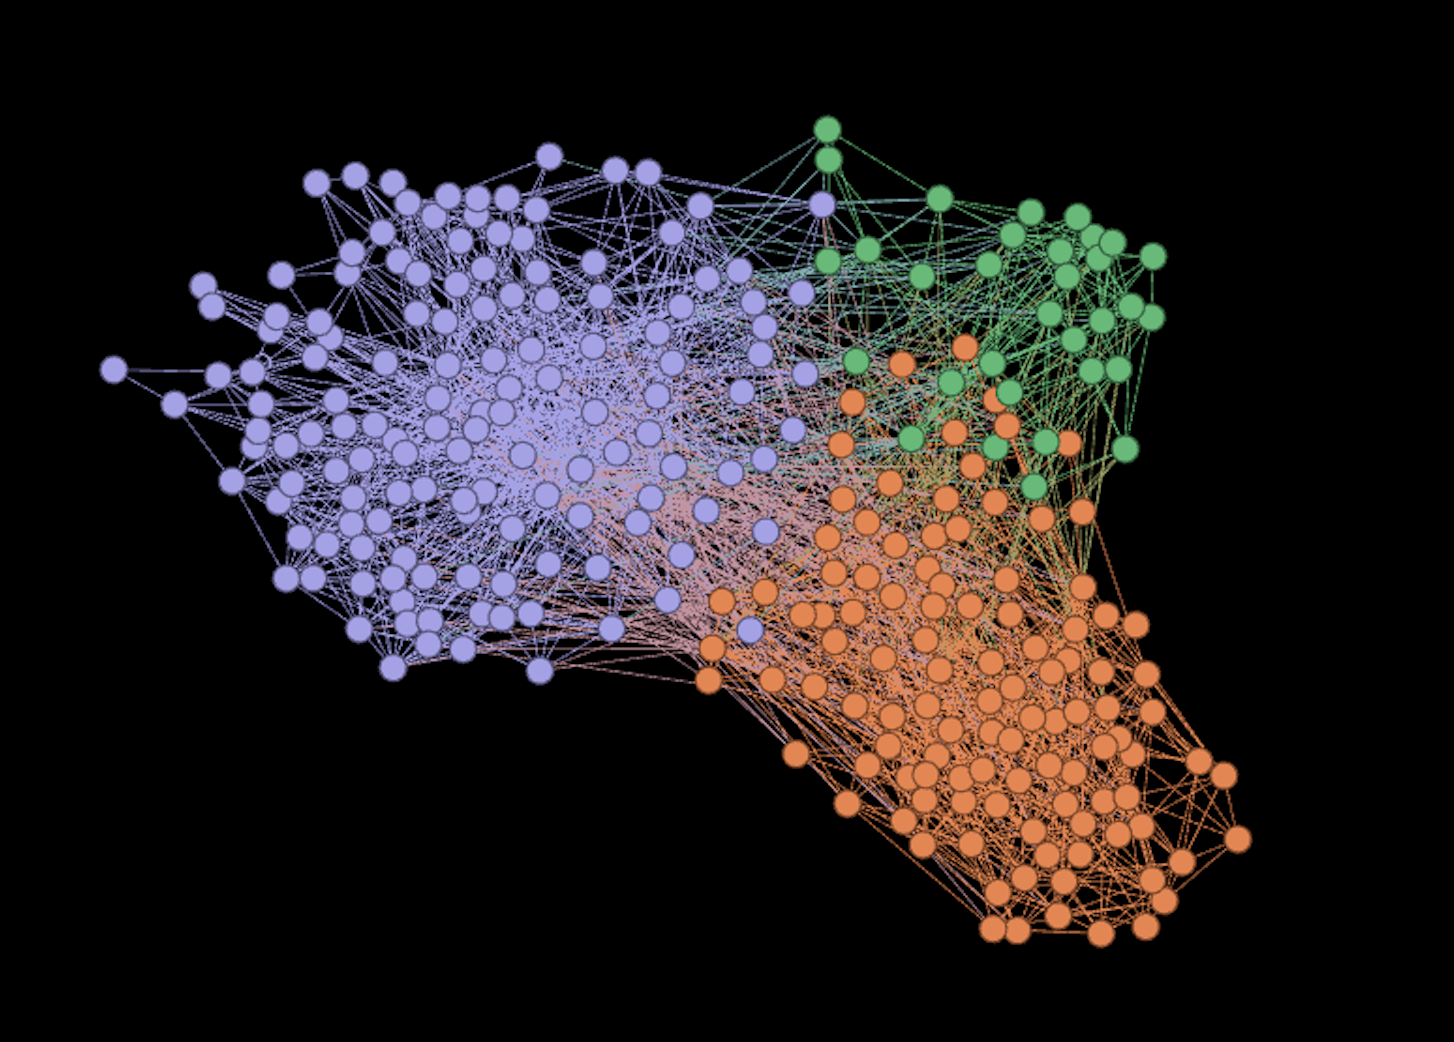
\includegraphics[width=0.28\textwidth]{c-elegans-k-means-zoomed.png}
    \caption{\begin{footnotesize}A visualization of the C. Elegans connectome partitioned using a graph autoencoder and k-means clustering, as performed in my CS 575 final course project. Partitions corresponded to sensory, motor, and interneuron divisions of the nervous system \end{footnotesize}}
    \label{fig:specific}

    \vspace{0.04\textwidth}

    \centering
    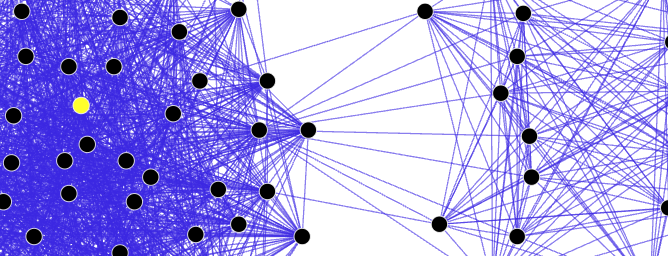
\includegraphics[width=0.28\textwidth]{social.png}
    \caption{\begin{footnotesize}Graph data science is applied to a diverse set of problems in domains including social science, information retrieval, and pharmaceutical development. Image courtesy of: \cite{darwinpeacock2014social, wikipedia2025social} \end{footnotesize}}
    \label{fig:general}
\end{wrapfigure}

The original method for collecting a connectome used a microscope, often implementing electron microscopy with computer-aided feature recognition of microscopy images \cite{white1986structure, emmons2015connectomics, bigbrain, sejnowski2016nanoconnectomics}. These assays provide excellent resolution, and can even give insight about extracellular context (e.g., supporting cells) but cannot be collected in-vivo and require significant tissue preparation ex-vivo. More recent (2010-2015) approaches have used fMRI and dMRI to collect human connectomes in-vivo \cite{elam2021hcp}. However, these MRI-based connectomes limit resolution to the voxel ($\approx1$mm 3D pixel) rather than to the cell. While not inhibiting association of brain regions to specific behaviors or other phenotypes, constrained resolution fails to measure essential nuance in processes between collections of cells inside each voxel. Additionally, the fMRI and dMRI techniques measure cellular activity only indirectly through mapping variables like blood flow, and cannot capture excitatory, inhibitory, or modulatory activity between cells necessary for precise characterization of inter-cellular relationships.

Simultaneous with these advancements in connectomics were developments in in-vivo electrophysiology approaches. Research-grade electrode probes (e.g., Neuropixels) have been developed to record the activity of multiple neurons from a single insertion point in in-vivo animal studies \cite{Jun2017, Paulk2022} and large-scale datasets have been collected for community use \cite{Laboratory2022, zhang2025neuralencodingdecodingscale}. In addition, medical devices have begun to be developed which will enable similar electrophysiology-based recording and stimulation of nervous tissue \cite{musk2019integrated, card2024neuroprosthesis, vilela2020bci}. Such devices have already shown promise in treating nervous system conditions ranging from quadriplegia to epilepsy \cite{vilela2020bci, geller2018responsive, Heck2014RNS}.

As a final and perhaps more obvious recent development, the last several years have shown explosive growth in machine learning research and commercialization, with the transformer model published in 2017 \cite{vaswani2023attentionneed} and diverse applications ranging from chatbots to protein structure prediction \cite{Jumper2021, wikipedia2025alphafold}. Additionally, complementary data science approaches have continued to develop, such as graph data science (e.g., \cite{velickovic2018graphattentionnetworks}, Figure \ref{fig:general}). Further, the body of research applying graph and similar data science approaches to connectomics is small relative to each respective field. The recent and concurrent progress in all these fields (connectomics, electrophysiology, brain computer interfaces, and data science/machine learning), as well as the apparent/potential lack of computational methodologies is processing this data, serves as inspiration for this master's project, and the beginning of my post-master's research portfolio.

\sectionwithindent{Objectives and Deliverables}
% - A list of deliverables to be considered in determining a grade (e.g. written and verbal reports, software, experimental results)
While making a significant research grade contribution in this space will be beyond the scope of this masters project, I aim to replicate existing scientific methods and refine my understanding of these field. I will do this by pursuing the following objectives and creating associated deliverables. I will work on the most basic objectives first, and complete as many of the objectives as my time constraints for the project allow.

\begin{enumerate}
    \item (Objective) Increase understand of (a) basic neural signal processing, (b) current approaches for electrophysiology data processing and (c) general principles for existing related work in micro-connectomics.
    \begin{itemize}
        \item (Deliverable) A literature review of works related to the topics introduced in this proposal (2-3 pages).
        \item (Deliverable) A revised/forked python package based on the International Brain Lab electrophysiology data processing python package(s), with a jupyter notebook tutorial demonstrating the neural signal processing tools.
    \end{itemize}

    \item (Objective) Implement and experiment with 3-5 algorithms for electrophysiology-based identification of connectome subgraphs with International Brain Lab small animal data \cite{Laboratory2022, zhang2025neuralencodingdecodingscale}. We will plan for algorithms to emphasize (a) pairwise statistics, (b) graph convolutional networks, and/or (c) other methods identified by literature review during (1).
    \begin{itemize}
        \item (Deliverable) A set of python classes and/or modules, and a jupyter notebook demonstrating these algorithms.
        \item (Stretch Deliverable) A report of test results with metrics for time-efficiency and reliability for each algorithm*.
    \end{itemize}

    \item (Stretch Objective) If resources allow, develop a visualization of the identified connectome subgraphs, potentially including dynamic firing patterns*.
    \begin{itemize}
        \item (Stretch Deliverable) A simulation or visualization (such as with Matplotlib or PyQT) of the identified subgraphs and any associated dynamics*.
    \end{itemize}

    \item (Objective) Demonstrate clear and professional communication in written and verbal format in reporting on this project.
    \begin{itemize}
        \item (Deliverable) A written report summarizing (a) results and conclusions related to the above objectives, (b) skills developed from this work, and (c) key takeaways to carry into future work (2-3 pages).
        \item (Deliverable) A brief presentation highlighting this project to be shared in-person with professors at the end of the project.
    \end{itemize}
\end{enumerate}
*These stretch objectives/deliverables are most ambitious, and may be removed from scope (or iterated on) depending on time constraints of the project.

\sectionwithindent{Plan for Weekly Meetings}
% - A plan for weekly meetings with the faculty advisor (e.g. weekly meetings at a specific time)
Dr. Goodrich and I will plan to meet at his office weekly on Tuesdays at 1:00 PM to review the status of this project, troubleshoot roadblocks, and plan iterative progress related to the project's questions and deliverables during Spring and Summer (2025) terms.

\sectionwithindent{Two-Sentence Summary}
The objective of this project is for me to understand data science central to the fields of connectomics, electrophysiology, and brain computer interfaces in order to prepare for successful admission to and graduation from a PhD program in neuroscience that emphasizes data science methods in these domains. I see that these fields have shown significant developments in recent years and show promise for future growth and applicability in coming years.

\sectionwithindent{One-Sentence Summary}
I am working to understand electrode-based recording of the brain and use it to build a network of neurons and computationally analyze the brain's function.

\newpage
\printbibliography

\end{document}
